\chapter{Experimental settings}

\paragraph{}
The different research that we analyzed and the purpose of our research drive us to focus our interest on the design of the application. As we mentioned earlier, Twitter changed its design in April in order to increase the engagement of its users. We noticed that the design was inspired by the Facebook one. We chose to simplify the design of the application and then reduce the overload of information as much as possible in order to avoid background noise, which would be difficult to measure. For this, we modeled after Tinder, an application where the user classifies females and males according to their physical appearance. We kept this classification workflow and improved the lock and field in order to easily identify our two metrics: engaged time and interest.\\
This section will be separated into two parts, where we will present and explain our design in one section and discuss the data acquisition in the other.

\section{The design}

\paragraph{}
Our protocol described last chapter did not include the design of the application. It gave us the metrics of engaged time and interest. The general workflow of the application is dictated by the A/B test, the design of the apps is the only remaining task that we need to develop. In order to collect data and measure user behaviours without noise, we start thinking as simple as possible. The two aspects of Twinder are to visualise and classify tweets exactly like Tinder. As you can see on picture \ref{fig:tinder}, the priority of the mobile application is the picture display. Two buttons are at the bottom of the page in order to classify the individual. When the user clicks on one of the buttons, the next profile appears and so on. Tinder is composed of three items: two buttons and a stack of pictures. \\

\begin{figure}[h] 
\centering 
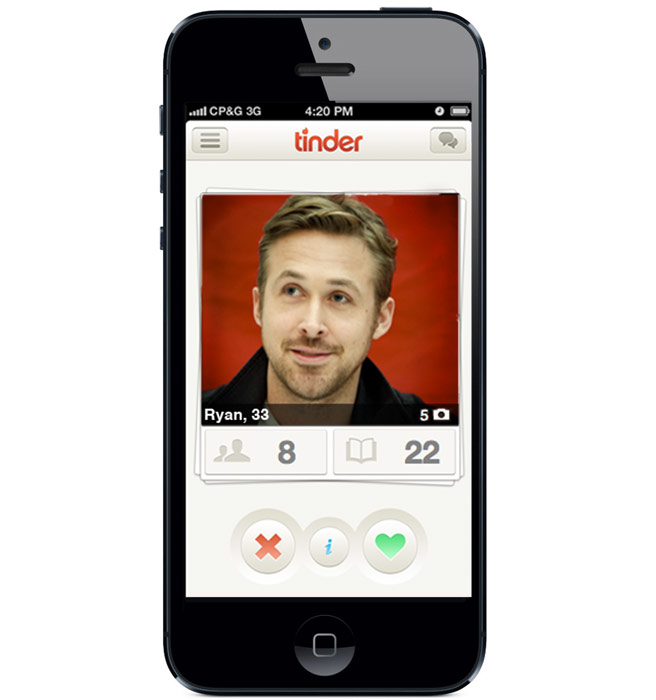
\includegraphics[width=0.3\columnwidth]{experiment_settings/tinder} 
\caption[Time spent of Social Media]{This clock shows the distribution of an hour online spent by US people. 16 min are on social network and forum. Source: \cite{s_clock}}
\label{fig:tinder} 
\end{figure}

Twinder is based on the same logic as Tinder, we keep the same three items: two buttons, but we change the stack of pictures into a stack of tweets. As we developed our apps for a laptop, we used the keyboard to take the input of the users. There was no need to display the two like / dislike buttons on the screen. To resume, we have a simple screen where the user visualizes tweets one after another by pressing two buttons. These buttons are two keyboard keys: L for like and D for dislike.\\
As you can see in the picture, we succeeded in retrieving the embedded tweets. We mentioned in the methodology section that the users need a context to more clearly understand these short messages of 140 charts. The embed format allows us to display the same content as one sees on Twitter, especially the images and other content, which is not only text.\\
We created a simple design for a simple action: classifying tweets. We developed an easy-to-use platform, which leads to a few random parameters that are difficult to evaluate. In order to control in a better way these few factors, we will describe the data acquisition process.

\section{Data acquisition}

The data acquisition was done in two steps. First, we did a beta test with 3 people and then performed the test on 15 people. \\
The beta test provided global feedback of the experiment and that allowed us to improve the application and survey. A sociology student advised us on how formulate our users' instructions without a clear bias or influence. \\
After doing this beta test, we ran a 15 experiences a day. Fifteen users took the same test A. Eight of them did test-time-B while the rest did test-like-B. All candidates shared similar profiles. They were all entrepreneurs working at 500 Startups, one of the biggest incubators in San Francisco. Each test subject had comprehensive understanding of Twitter and the popular new media. An unexpected result of this project showed that people from across the world do not use Twitter in the same way.\\
The test was administered in a quiet conference room at the 500 startup office. \\ \\ \\ \\ \\ \\
The candidates took the test individually and received test A simple instructions at the start of the experiment:

\begin{itemize}
  \item \textbf{Press L} if you find the content of the tweet interesting.
  \item \textbf{Press D} if you do not find the content of the tweet interesting.
  \item Take your time to do the test.
\end{itemize}

 


Once the user finished test A, we talked to the user in to try and change their mind. After our conversation,each user would then start test B and finish the survey.
Moving forward from the explanation of the experimental setting, we will now define the technical implementation of Twinder.
